\documentclass[codesnippet]{jss}

%% -- LaTeX packages and custom commands ---------------------------------------

%% recommended packages
\usepackage{thumbpdf,lmodern}

%% another package (only for this demo article)
\usepackage{framed}

%% new custom commands
\newcommand{\class}[1]{`\code{#1}'}
\newcommand{\fct}[1]{\code{#1()}}


%% -- Article metainformation (author, title, ...) -----------------------------

%% - \author{} with primary affiliation
%% - \Plainauthor{} without affiliations
%% - Separate authors by \And or \AND (in \author) or by comma (in \Plainauthor).
%% - \AND starts a new line, \And does not.
\author{Elan Ness-Cohn\\Northwestern University
   \And Rosemary Braun\\Northwestern University}
\Plainauthor{Elan Ness-Cohn, Rosemary Braun}

%% - \title{} in title case
%% - \Plaintitle{} without LaTeX markup (if any)
%% - \Shorttitle{} with LaTeX markup (if any), used as running title
\title{Fasano Franceschini Test: an Implementation of a 2-Dimensional Kolmogorov--Smirnov in \proglang{R}}
\Plaintitle{Fasano Franceschini Test: an Implementation of a 2-Dimensional Kolmogorov--Smirnov in R}
\Shorttitle{2-Dimensional Kolmogorov--Smirnov in \proglang{R}}

%% - \Abstract{} almost as usual
\Abstract{
The \pkg{fasano.franceschini.test} package is an  \proglang{R} implementation of the 2-D Kolmogorov-Smirnov (KS) two--sample test as defined by Fasano and Franceschini \citep{Fasano1987}. This is a variant of the 2-D two-sample KS test as originally defined by Peacock \citep{Peacock1983}, previously implemented in \proglang{R} in the \pkg(Peacock.test) package \citep{Xiao2016}. The \pkg{fasano.franceschini.test} package provides a two fold improvement over the current 2-D KS test on the Comprehensive \proglang{R} Archive Network (CRAN): \textbf{(i)} The Fasano and Franceschini test has been shown to run in $O(n^2)$ versus the Peacock implementation which runs in $O(n^3)$. \textbf{(ii)} The package implements a  bootstrapping procedure for improved significance testing.
}

%% - \Keywords{} with LaTeX markup, at least one required
%% - \Plainkeywords{} without LaTeX markup (if necessary)
%% - Should be comma-separated and in sentence case.
\Keywords{Fasano--Franceschini test, 2-D Kolmogorov--Smirnov test, Multivariate, KS test, \proglang{R}}
\Plainkeywords{Fasan--Franceschini test, 2-D Kolmogorov--Smirnov test, Multivariate, KS test,  R}

%% - \Address{} of at least one author
%% - May contain multiple affiliations for each author
%%   (in extra lines, separated by \emph{and}\\).
%% - May contain multiple authors for the same affiliation
%%   (in the same first line, separated by comma).
\Address{
  Elan Ness-Cohn\\
  Department of Molecular Biosciences,\\
  Biostatistics Division of The Department of Preventive Medicine,\\
  \emph{and}\\
  NSF-Simons Center for Quantitative Biology\\
  Northwestern University\\
  Evanston, IL 60208\\
  E-mail: \email{elan.ness-cohn@northwestern.edu}\\
  URL: \url{https://sites.northwestern.edu/elannesscohn/}\\

Rosemary Braun\\
  Department of Molecular Biosciences,\\
  Biostatistics Division of The Department of Preventive Medicine,\\
  NSF-Simons Center for Quantitative Biology,\\
  Department of Engineering Sciences and Applied Mathematics,\\
  Department of Physics and Astronomy,\\
  \emph{and}\\
  Northwestern Institute on Complex Systems\\
  Northwestern University\\
  Evanston, IL 60208\\
  E-mail: \email{rbraun@northwestern.edu}\\
  URL: \url{https://sites.northwestern.edu/braunlab/}\\

}
\begin{document}


%% -- Introduction -------------------------------------------------------------

%% - In principle "as usual".
%% - But should typically have some discussion of both _software_ and _methods_.
%% - Use \proglang{}, \pkg{}, and \code{} markup throughout the manuscript.
%% - If such markup is in (sub)section titles, a plain text version has to be
%%   added as well.
%% - All software mentioned should be properly \cite-d.
%% - All abbreviations should be introduced.
%% - Unless the expansions of abbreviations are proper names (like "Journal
%%   of Statistical Software" above) they should be in sentence case (like
%%   "generalized linear models" below).

\section[Introduction]{Introduction} \label{sec:intro}

% R -> Peacock test (computationally inificent)
% Python <- Implementation
% C <- Implementation

The Kolmogorov--Smirnov (KS) is a non--parametric, univariate statistical test designed to assess whether a set of data is consistent with a given probability distribution. First derived by Kolmogorov and Smirnov in a series of papers~\citep{Kolmogorov1933,Kolmogorov1933a,Smirnov1936,Smirnov1937,Smirnov1939,Smirnov1944,Smirnov1948}, the one-sample KS test defines the distribution of the quantity $D_{KS}$ -- the maximal absolute difference between the empirical cumulative distribution function of a set of values and a reference probability distribution. Kolmogorov and Smirnov's key insight was proving the distribution of the quantity $D_{KS}$ to be distribution free -- meaning the distribution does not depend on the underlying cumulative distribution functions being tested. Thus, the test can effectively be used to compare any univariate empirical data distribution to any continuous univariate reference distribution. A similar two-sample KS test could further be used to compare any two univariate empirical data distributions against each other to determine if they are drawn from the same underlying univariate distribution.

The versatility of the univariate KS test has made it a cornerstone of statistical analysis and is commonly used across the scientific disciplines(Cite uses in a broad range of field). Nonetheless, a generalization of the KS test as proposed by Kolmogorov and Smirnov does not naturally extend when working with data in more than one dimension. Fortunately, a solution to the dimensionality issue was articulated by Peacock \citep{Peacock1983} and later extended by Fasano and Franceschini \citep{Fasano1987}.

Currently, only the Peacock implementation of the 2-D two-sample KS test is available in \proglang{R} \citep{R} with the \pkg{Peacock.test} package via the \fct{peacock2} function; and has been shown to be markedly slower than the Fasano and Franceschini algorithm\citep{Lopes2007}. A \proglang{C} implementation of the Fasano Franceschini test is available in \citep{numericalRecipes}; however, arguments have been made to the validity of the implementation of the test not being distribution-free\citep{Babu2006}. Furthermore, the \proglang{C} implementation statistical testing is based on a fit to Monte Carlo Simulation and is only valid if the indicated probability (significance level) is less than (more significant than) $\sim 0.20$, which may present potential issues in some analysis.

Here we present the \pkg{fasano.franceschini.test} package as an \proglang{R} implementation of the 2-D two-sample KS test as defined by Fasano and Franceschini \citep{Fasano1987} The \pkg{fasano.franceschini.test} package provides a two fold improvement over the current 2-D KS test on the Comprehensive \proglang{R} Archive Network (CRAN): \textbf{(i)} The Fasano and Franceschini test has been shown to run in $O(n^2)$ versus the Peacock implementation which runs in $O(n^3)$. \textbf{(ii)} The package implements a bootstrapping procedure for improved significance testing and mitigates the concerns over the distribution-free nature of the test brought up by\citep{Babu2006}.


% \begin{leftbar}
% The introduction is in principle ``as usual''. However, it should usually embed
% both the implemented \emph{methods} and the \emph{software} into the respective
% relevant literature. For the latter both competing and complementary software
% should be discussed (within the same software environment and beyond), bringing
% out relative (dis)advantages. All software mentioned should be properly
% \verb|\cite{}|d. (See also Appendix~\ref{app:bibtex} for more details on
% \textsc{Bib}{\TeX}.)
%
% For writing about software JSS requires authors to use the markup
% \verb|\proglang{}| (programming languages and large programmable systems),
% \verb|\pkg{}| (software packages), \verb|\code{}| (functions, commands,
% arguments, etc.). If there is such markup in (sub)section titles (as above), a
% plain text version has to be provided in the {\LaTeX} command as well. Below we
% also illustrate how abbrevations should be introduced and citation commands can
% be employed. See the {\LaTeX} code for more details.
% \end{leftbar}
%
% Modeling count variables is a common task in economics and the social sciences.
% The classical Poisson regression model for count data is often of limited use in
% these disciplines because empirical count data sets typically exhibit
% overdispersion and/or an excess number of zeros. The former issue can be
% addressed by extending  the plain Poisson regression model in various
% directions: e.g., using sandwich covariances or estimating an additional
% dispersion parameter (in a so-called quasi-Poisson model). Another more formal
% way is to use a negative binomial (NB) regression. All of these models belong to
% the family of generalized linear models (GLMs). However, although these models
% typically can capture overdispersion rather well, they are in many applications
% not sufficient for  modeling excess zeros. Since \cite{Mullahy:1986} there is
% increased interest in zero-augmented models that address this issue by a second
% model component capturing zero counts. An overview of count data models in
% econometrics, including  hurdle and zero-inflated models, is provided in
% \cite{Cameron+Trivedi:2013}.
%
% In \proglang{R} \citep{R}, GLMs are provided by the model fitting functions
% \fct{glm} in the \pkg{stats} package and \fct{glm.nb} in the \pkg{MASS} package
% \citep[][Chapter~7.4]{Venables+Ripley:2002} along with associated methods for
% diagnostics and inference. The manuscript that this document is based on
% \citep{Zeileis+Kleiber+Jackman:2008} then introduced hurdle and zero-inflated
% count models in the functions \fct{hurdle} and \fct{zeroinfl} in the \pkg{pscl}
% package \citep{Jackman:2015}. Of course, much more software could be discussed
% here, including (but not limited to) generalized additive models for count data
% as available in the \proglang{R} packages \pkg{mgcv} \cite{Wood:2006},
% \pkg{gamlss} \citep{Stasinopoulos+Rigby:2007}, or \pkg{VGAM} \citep{Yee:2009}.


%% -- Manuscript ---------------------------------------------------------------

%% - In principle "as usual" again.
%% - When using equations (e.g., {equation}, {eqnarray}, {align}, etc.
%%   avoid empty lines before and after the equation (which would signal a new
%%   paragraph.
%% - When describing longer chunks of code that are _not_ meant for execution
%%   (e.g., a function synopsis or list of arguments), the environment {Code}
%%   is recommended. Alternatively, a plain {verbatim} can also be used.
%%   (For executed code see the next section.)

\section{Models and software} \label{sec:models}

\subsection{1-D Kolmogorov--Smirnov Test}

The Kolmogorov--Smirnov (KS) test is a non--parametric method for determining where a sample is consistent with a given probability distribution. While a comprehensive discussion pertaining the intricacies of the 1-D KS test can be found elsewhere~\citep{Stephens1992a}, we will present a brief overview as motivation for the basis and intuition of the 2-D KS test.

As described previously, the 1-D KS test can be divided into two variants of the same statistical procedure:

\begin{leftbar}
\textbf{The One-Sample Test}
\begin{itemize}
\item Compares the data to an analytical distribution.
\end{itemize}
\textbf{The Two-Sample Test}
\begin{itemize}
\item Compares two data samples to determine if they are drawn from the same underlying probability distribution.
\end{itemize}
\end{leftbar}

In both cases, the KS test works as follows:

The Kolmogorov-Smirnov statistic (D) is the defined by the maximum absolute difference between the cumulative density functions of the data and model (one--sample), or between the two data sets (two--sample). In the following example, the orange and blue curve in the left panel represents the underlying distribution (pdf) for sample1 and sample2, respectively (\textbf{Figure \ref{fig:kstest1D}}). The eCDF is then defined by data drawn from these underlying distribution, and the D--stat is the computed as the largest between difference between the eCDF (black dotted line) in the right panel.

\begin{figure}[t!]
\centering
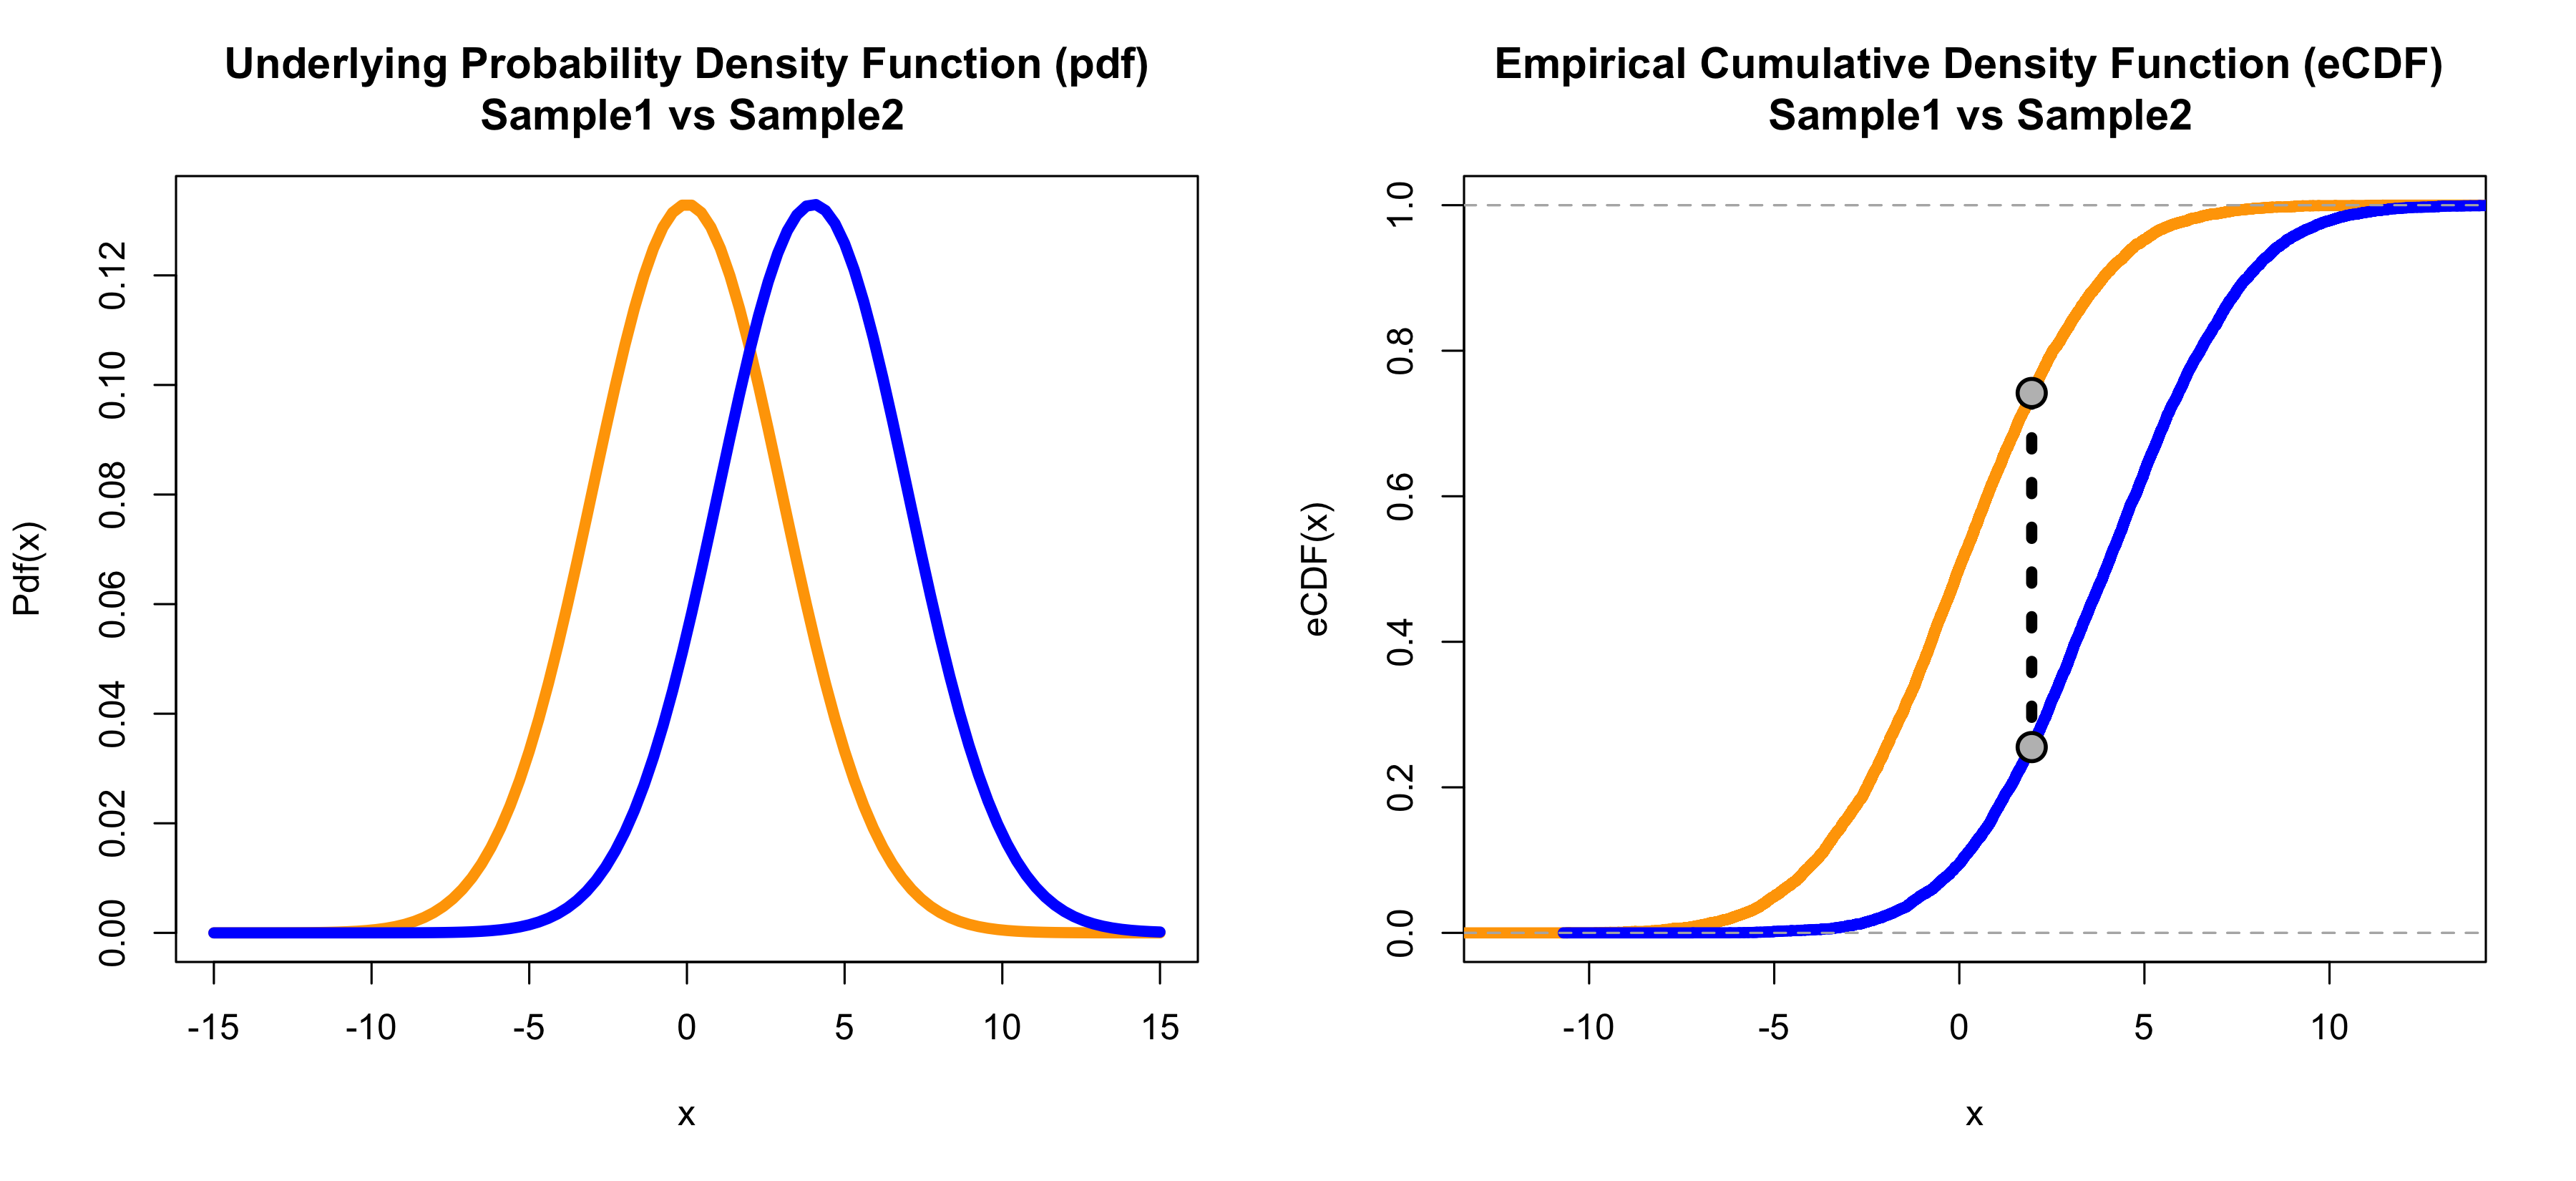
\includegraphics{pdfvsCDF}
\caption{\label{fig:kstest1D} \textbf{LEFT:} Probability density function (PDF) of two normal distribution: orange sample1 $\mathcal{N}(\mu = 0,\,\sigma^{2} = 1)$; blue sample2 $\mathcal{N}(\mu = 5,\,\sigma^{2} = 1)$. \textbf{RIGHT:} Empirical cumulative density functions (eCDF) of the two PDFs in the left panel. Black dotted line represents the maximal absolute difference between the eCDFs ($D_{KS}$).
}
\end{figure}

Kolmogorov and Smirnov work mathematically defined the distribution for D to be distribution free, and further derived a table of critical values for hypothesis testing. Kolmogorov and Smirnov work was later refined by Kendall and Stuart ~\citep{Kendall1946} to define the integrated probability distribution for large values of n  ($n \geq 80$), having the asymptotic expression:

\begin{equation} \label{eq:1}
\Phi(\lambda) = 2 \sum_{k=1}^{\infty} -1^{k-1}e^{-2k^2\lambda^2}
\end{equation}

Given the maximum absolute difference (D) and \textbf{Equation~\ref{eq:1}}, one can  compute a $p$-value for  hypothesis testing to determine if there is a significance difference between the cumulative density functions of the data and model (one-sample), or between the two data sets (two-sample).

\textbf{For the 1-Sample case}, the $p$-value probability of a given D-stat is defined by

\begin{equation} \label{eq:2}
Prob(D > observed) = \Phi ( D\sqrt{N})
\end{equation}

where $N$ is the number of data points sampled. A $p$-value $< 0.05$, indicates a significant difference between the samples.

\textbf{In the 2-Sample case}, the $p$-value probability of a given D-stat is defined by
\begin{equation} \label{eq:3}
Prob(D > observed) = \Phi ( D\sqrt{\frac{n_1n_2}{n_1+n_2}})
\end{equation}

where $n_1$ and $n_2$ is the number of data points in the first and second samples respectively. A $p$-value $< 0.05$, indicates a significant difference between the samples.

\subsection{Higher Dimensional KS Test}

Similar to the 1-D KS test, the obvious solution to extend the theory into higher dimensional would be to define the maximal cumulative difference between the two 2-D distributions. This however, presents an issue as the commutative distribution function is not well defined in more than one dimension. In 2-D, there are 4 ways (3 independent ways) of defining the cumulative distribution, since the direction in which we define choose to order the points in the x and y are arbitrary (\textbf{Figure \ref{fig:kstest2Dissue}}). In N dimensional space there are $2^{N}-1$ independent ways of defining the cumulative distribution function~\citep{Peacock1983}.


\begin{figure}[t!]
\centering
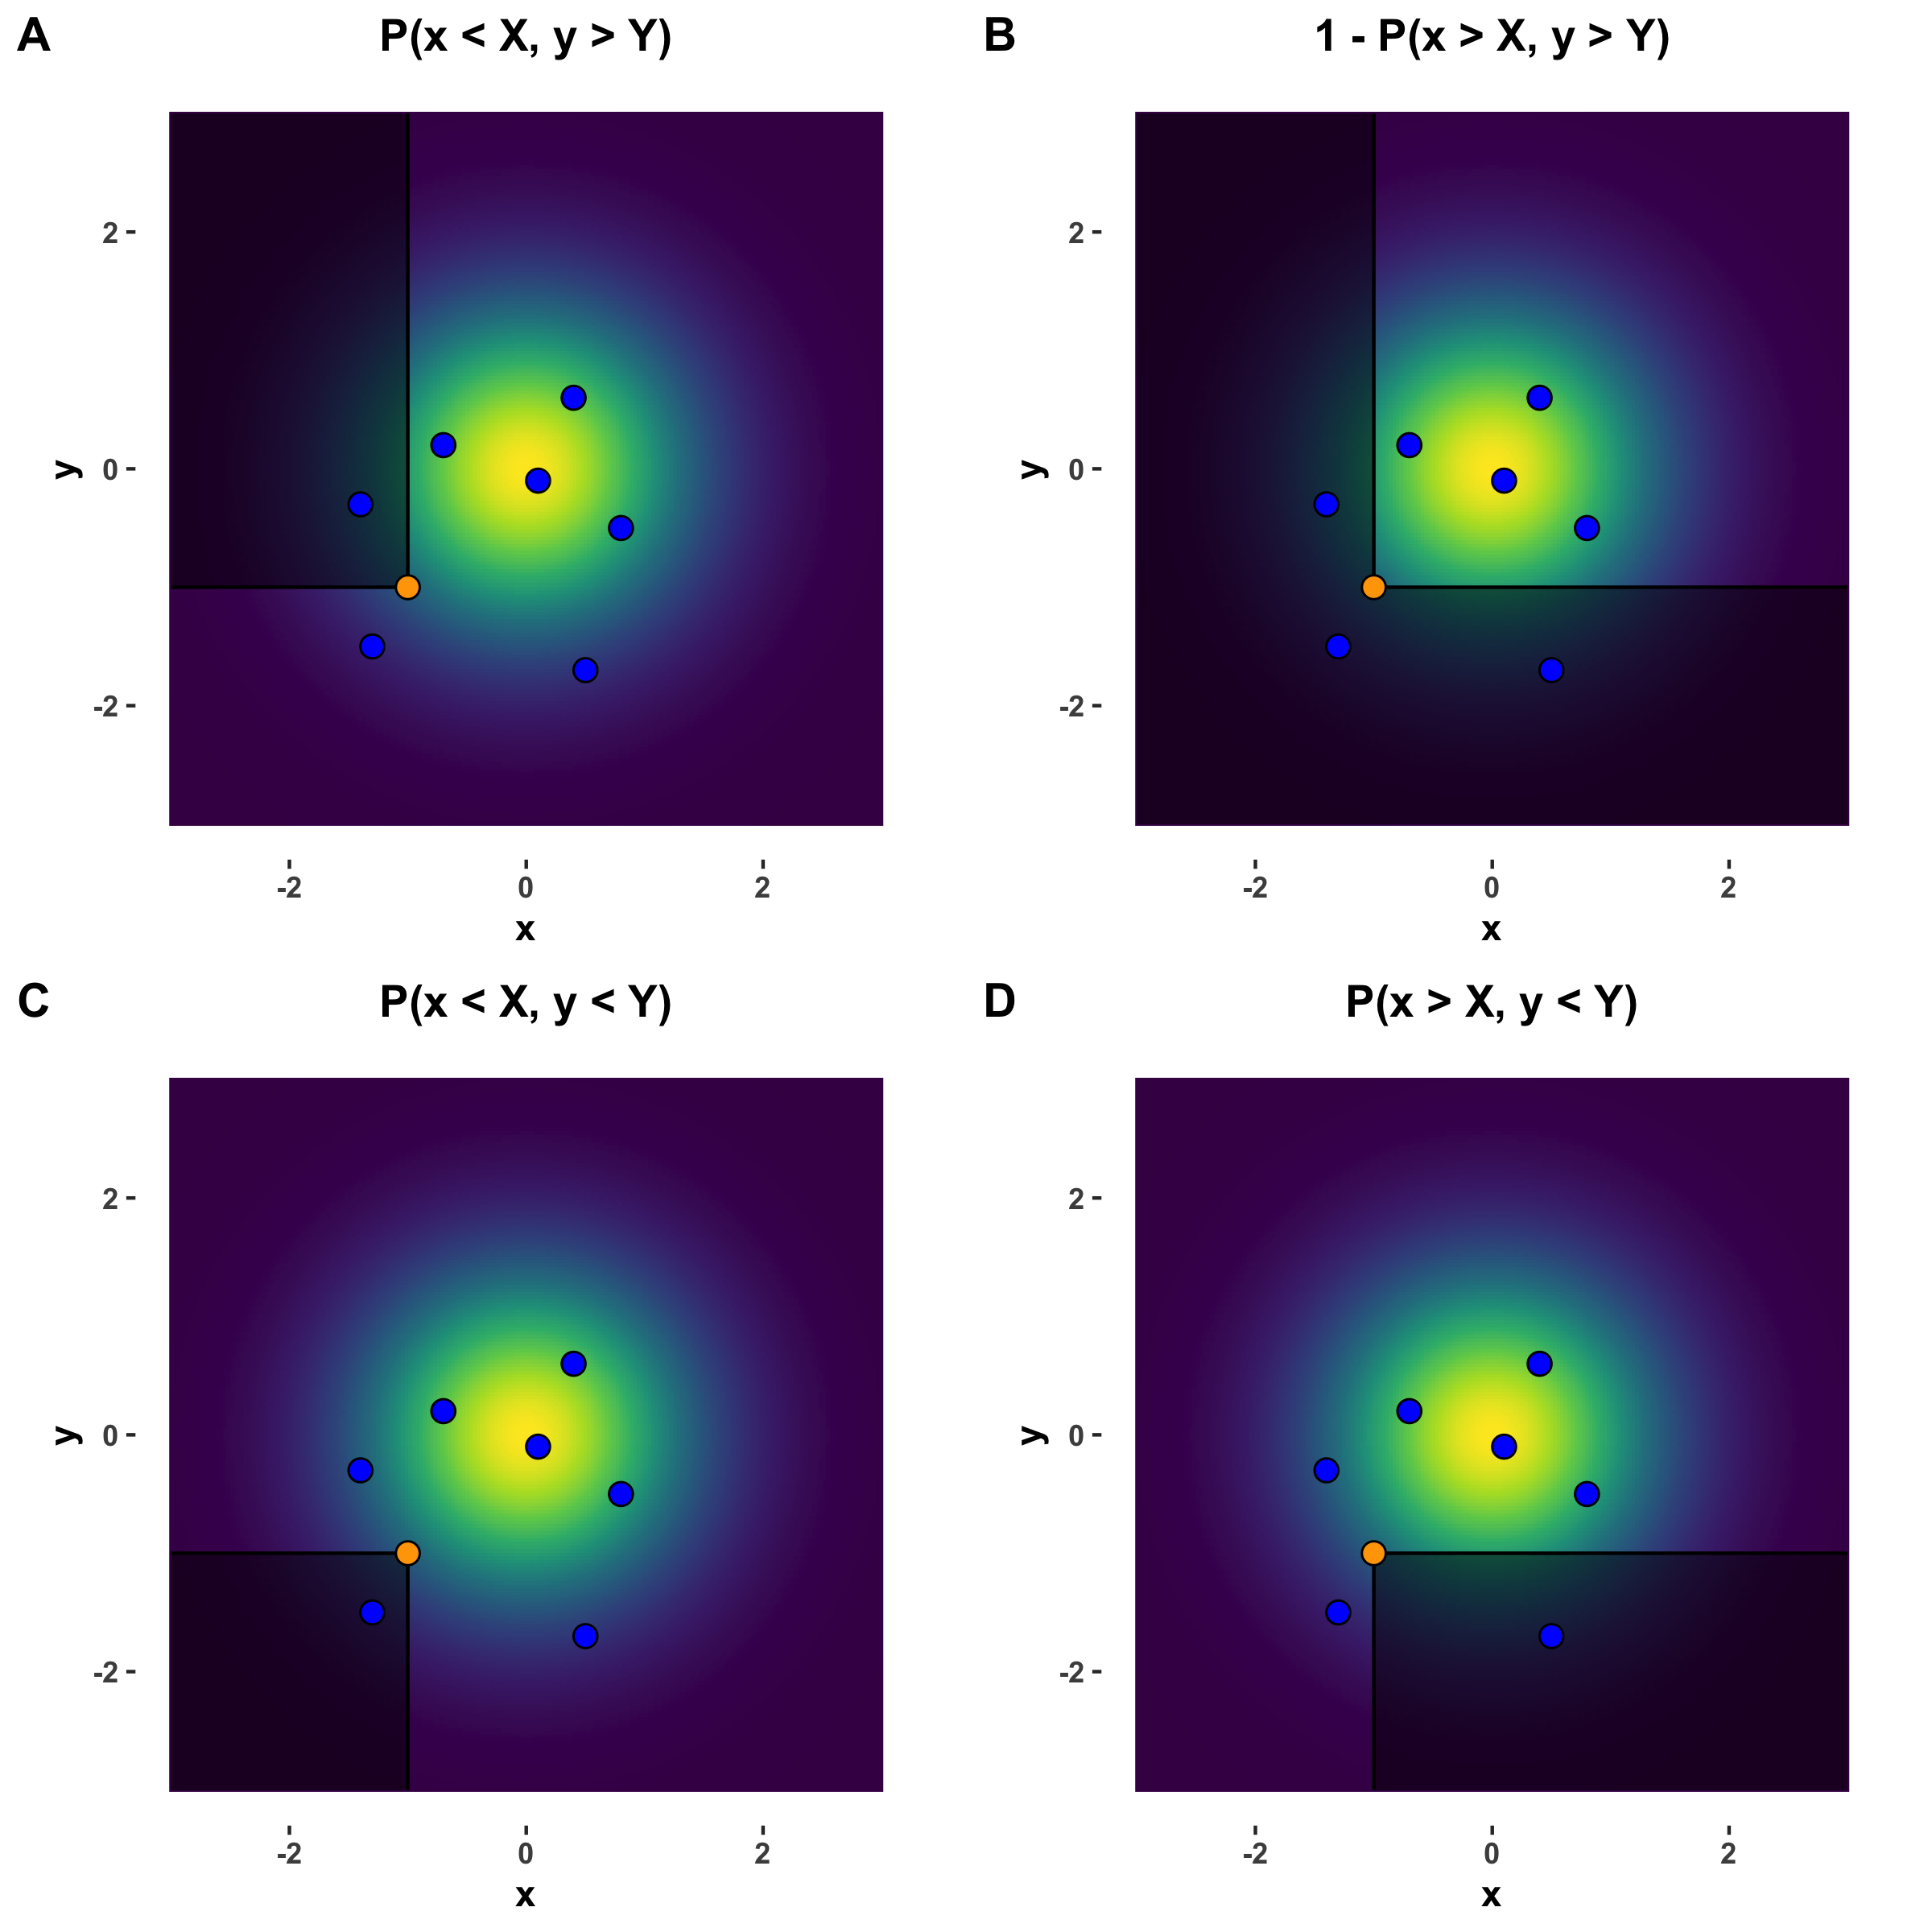
\includegraphics{CDF2Dissue}
\caption{\label{fig:kstest2Dissue} 4 ways (3 independent ways) of defining the cumulative distribution for a given point in 2-D.
$P(x < X, y < Y) + P(x < X, y > Y) + P(x > X, y < Y) = 1 - P(x > X, y > Y)$}
\end{figure}

\subsection{Peacock Test (1983) and Fasano Franceschini Test (1987)}
Peacock solved the higher dimensionality issue by defining the 2-D test statistic as the largest difference between the empirical and theoretical commutative distributions, after taking all possible ordering combinations into account. Peacock test thus computes the total integrated probability -- i.e. fraction of data -- in each of the four quadrants around all possible points in the data. For example, for a given $n$ points in a two-dimensional space, the cumulative distribution functions is calculated in the $4n^2$ quadrants of the plane defined by all pairs ($X_i$ ,$Y_j$), $X_i$ and $Y_j$ being coordinates of any pairs of points in the given sample. By ranging over all possible pairs of data points and quadrants, the 2-D D-stat is defined by the maximal difference of the integrated probabilities between samples.

The slight variation defined by Fasano and Franceschini was to only consider quadrants centered in each point of the given samples to compute the cumulative distribution functions. e.g, rather than looking over all ($X_i$ ,$Y_j$; where $i,j={1,n}$), Fasano and Franceschini only used the detected points ($X_i$ ,$Y_i$; where $i={1,n}$). Thus for an given $n$ points in a two-dimensional space, those $n$ points define $4n$ -- rather than $4n^2$ -- quadrants.

The 2-D two sample Fasano and Franceschini test is illustrated in the following example to compare the 2-D distributions of orange versus blue points (\textbf{Figure \ref{fig:kstest2D}}).

\begin{figure}[t!]
\centering
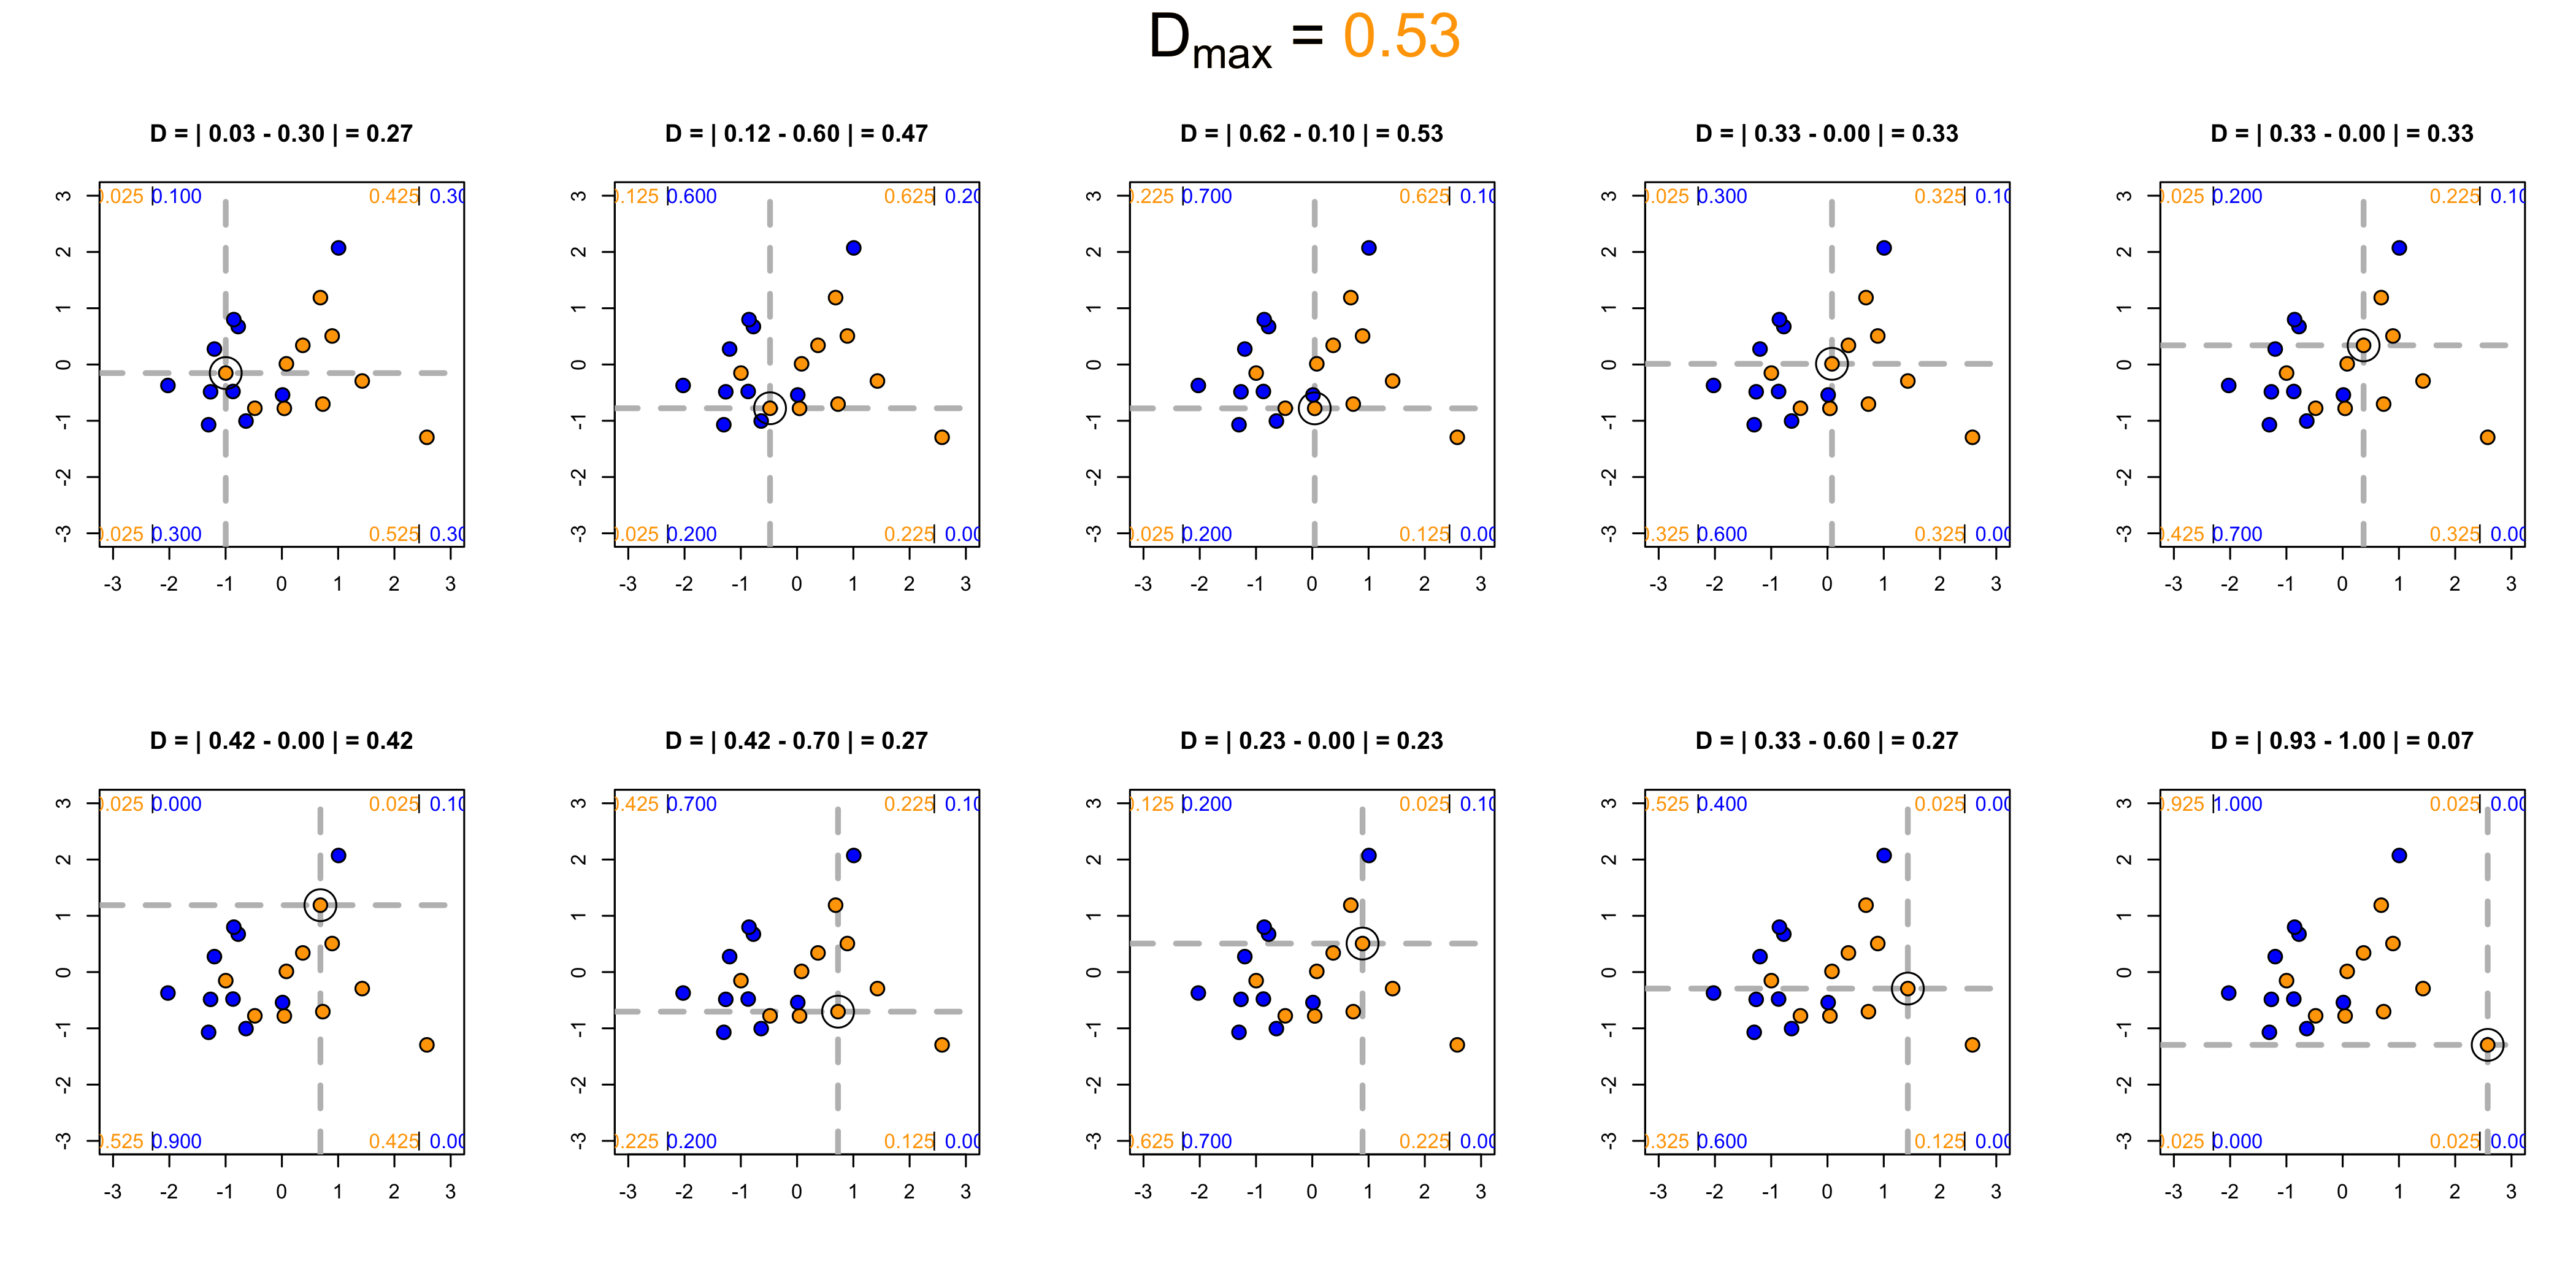
\includegraphics{fftestOutput}
\caption{\label{fig:kstest2D} Illustration of the Fasano Franceschini algorithmic search for the maximal difference (D) between sample 2-D eCDFs. Looping through each point in the sampled data to define a unique origin (grey dotted line), the fraction of orange and blue points in each quadrants are computed (plot corners). For each origin, the quadrant which maximizes the absolute difference in the integrated probabilities is indicated. The origin which maximizes the overall absolute difference in the integrated probabilities between samples is highlighted by the orange box.
}
\end{figure}

The algorithm loops through each point in the orange sample in turn to define the origin of 4 quadrants (grey dotted line). The fraction of orange and blue points in each quadrant is computed (corners of plot) and the quadrant with the maximal difference is designated with the current maximum for the specified origin. By ranging over all pairs of data points and quadrants, the 2-D D-stat is defined by the maximal difference of the integrated probabilities between samples. In this case using the orange point as the origin, the maximal difference is $D = 0.60$.

This process is repeated using the blue points as the origins to compute the maximal D-stat. Finally, both maximal D-stats using the orange and blue points as origins are then averaged to compute the overall D-stat for hypothesis testing.

\subsection{Defining the Fasano and Franceschini Null Distribution}

Using Monte Carlo simulation, Fasano and Franceschini created a series of critical value look up tables of values of D -- as a function of $D$, the sample size $N$, and the coefficient of correlation $r$. Teukolsky and Press later defined an approximate fit to this data in equation \ref{eq:4} for quick computation \cite{numericalRecipes}.

\textbf{For the 1-Sample case}

\begin{equation} \label{eq:4}
Prob(D > observed) = \Phi ( \frac{D\sqrt{N}}{1+\sqrt{1-r^2}(0.25-0.75/\sqrt{N})})
\end{equation}

\textbf{The 2-Sample case}

Uses the same formula as above, but with the slight variation where

\begin{equation} \label{eq:5}
N = \frac{n_1n_2}{n_1+n_2}
\end{equation}

In both cases, $r$ is defined by:

\begin{equation} \label{eq:6}
r = \frac{\sum_{i}^{}(x_i-\bar{x})(y_i-\bar{y})}{\sqrt{\sum_{i}^{}(x_i-\bar{x})^2}\sqrt{\sum_{i}^{}(y_i-\bar{y})^2}}
\end{equation}

% The basic Poisson regression model for count data is a special case of the GLM
% framework \cite{McCullagh+Nelder:1989}. It describes the dependence of a count
% response variable $y_i$ ($i = 1, \dots, n$) by assuming a Poisson distribution
% $y_i \sim \mathrm{Pois}(\mu_i)$. The dependence of the conditional mean
% $\E[y_i \, | \, x_i] = \mu_i$ on the regressors $x_i$ is then specified via a
% log link and a linear predictor
% %
% \begin{equation} \label{eq:mean}
% \log(\mu_i) \quad = \quad x_i^\top \beta,
% \end{equation}
% %
% where the regression coefficients $\beta$ are estimated by maximum likelihood
% (ML) using the iterative weighted least squares (IWLS) algorithm.
%
% \begin{leftbar}
% Note that around the \verb|{equation}| above there should be no spaces (avoided
% in the {\LaTeX} code by \verb|%| lines) so that ``normal'' spacing is used and
% not a new paragraph started.
% \end{leftbar}
%
% \proglang{R} provides a very flexible implementation of the general GLM
% framework in the function \fct{glm} \citep{Chambers+Hastie:1992} in the
% \pkg{stats} package. Its most important arguments are
% \begin{Code}
% glm(formula, data, subset, na.action, weights, offset,
%   family = gaussian, start = NULL, control = glm.control(...),
%   model = TRUE, y = TRUE, x = FALSE, ...)
% \end{Code}
% where \code{formula} plus \code{data} is the now standard way of specifying
% regression relationships in \proglang{R}/\proglang{S} introduced in
% \cite{Chambers+Hastie:1992}. The remaining arguments in the first line
% (\code{subset}, \code{na.action}, \code{weights}, and \code{offset}) are also
% standard  for setting up formula-based regression models in
% \proglang{R}/\proglang{S}. The arguments in the second line control aspects
% specific to GLMs while the arguments in the last line specify which components
% are returned in the fitted model object (of class \class{glm} which inherits
% from \class{lm}). For further arguments to \fct{glm} (including alternative
% specifications of starting values) see \code{?glm}. For estimating a Poisson
% model \code{family = poisson} has to be specified.
%
% \begin{leftbar}
% As the synopsis above is a code listing that is not meant to be executed,
% one can use either the dedicated \verb|{Code}| environment or a simple
% \verb|{verbatim}| environment for this. Again, spaces before and after should be
% avoided.
%
% Finally, there might be a reference to a \verb|{table}| such as
% Table~\ref{tab:overview}. Usually, these are placed at the top of the page
% (\verb|[t!]|), centered (\verb|\centering|), with a caption below the table,
% column headers and captions in sentence style, and if possible avoiding vertical
% lines.
% \end{leftbar}
%
% \begin{table}[t!]
% \centering
% \begin{tabular}{lllp{7.4cm}}
% \hline
% Type           & Distribution & Method   & Description \\ \hline
% GLM            & Poisson      & ML       & Poisson regression: classical GLM,
%                                            estimated by maximum likelihood (ML) \\
%                &              & Quasi    & ``Quasi-Poisson regression'':
%                                            same mean function, estimated by
%                                            quasi-ML (QML) or equivalently
%                                            generalized estimating equations (GEE),
%                                            inference adjustment via estimated
%                                            dispersion parameter \\
%                &              & Adjusted & ``Adjusted Poisson regression'':
%                                            same mean function, estimated by
%                                            QML/GEE, inference adjustment via
%                                            sandwich covariances\\
%                & NB           & ML       & NB regression: extended GLM,
%                                            estimated by ML including additional
%                                            shape parameter \\ \hline
% Zero-augmented & Poisson      & ML       & Zero-inflated Poisson (ZIP),
%                                            hurdle Poisson \\
%                & NB           & ML       & Zero-inflated NB (ZINB),
%                                            hurdle NB \\ \hline
% \end{tabular}
% \caption{\label{tab:overview} Overview of various count regression models. The
% table is usually placed at the top of the page (\texttt{[t!]}), centered
% (\texttt{centering}), has a caption below the table, column headers and captions
% are in sentence style, and if possible vertical lines should be avoided.}
% \end{table}


%% -- Illustrations ------------------------------------------------------------

%% - Virtually all JSS manuscripts list source code along with the generated
%%   output. The style files provide dedicated environments for this.
%% - In R, the environments {Sinput} and {Soutput} - as produced by Sweave() or
%%   or knitr using the render_sweave() hook - are used (without the need to
%%   load Sweave.sty).
%% - Equivalently, {CodeInput} and {CodeOutput} can be used.
%% - The code input should use "the usual" command prompt in the respective
%%   software system.
%% - For R code, the prompt "R> " should be used with "+  " as the
%%   continuation prompt.
%% - Comments within the code chunks should be avoided - these should be made
%%   within the regular LaTeX text.

\section{Illustrations} \label{sec:illustrations}

\subsection{Fasano Franceschini Test Usage}

In their paper, Fasano and Franceschini use Monte Carlo simulation to approximate the distribution of D as a function of $D$, the sample size $N$, and the coefficient of correlation $r$. Unlike the 1-D KS test, the 2-D KS test is not rigorously true that the distribution of D is independent of the shape of the 2-D distribution. Fasano and Franceschini reasoned that the coefficient of correlation between the two-dimensional distributions is what governs the resultant distribution of D. For example, if the data sets are perfectly correlated ($r = 1$), the 2-D plane flattens to a single line and thus a 1-D KS test could be used. If the data sets are perfectly uncorrelated ($r = 0$), the 2-D distribution is independent in the x and y directions and thus one could use a 1-D KS test on the marginal x or y distribution of the 2-D plane.
Results from Monte Carlo simulation support these assumptions -- showing that the distribution of D is nearly identical for varying distributions, assuming they have the same coefficient of correlation r ~\citep{Fasano1987}. The resultant distributional approximation fit by Teukolsky and Press -- as described above in equation \ref{eq:4} -- can be used to test the significance levels for the 2-D K-S test using the following code.

\begin{CodeChunk}
\begin{CodeInput}
R> #set seed for reproducible example
R> set.seed(123)
R>
R> #create 2-D samples with the same underlying distributions
R> sample1Data <- data.frame(
R>  x = rnorm(n = 100, mean = 0, sd = 1),
R>  y = rnorm(n = 100, mean = 0, sd = 1)
R> )
R> sample2Data <- data.frame(
R>  x = rnorm(n = 100, mean = 0, sd = 1),
R>  y = rnorm(n = 100, mean = 0, sd = 1)
R> )
R>
R> fasano.franceschini.test(sample1Data,sample2Data)
\end{CodeInput}
\begin{CodeOutput}
      2-D Two-sample Kolmogorov-Smirnov Test

 Fasano Franceschini Test (1987)
 Data:  sample1Data and sample2Data
 D-stat =  0.14 , p-value =  0.4420642
 Run Time (s) =  0.04288507
\end{CodeOutput}
\end{CodeChunk}

\subsection{Bootstrap Version of the Fasano Franceschini Test}

As a caveat, to the fit produced by Teukolsky and Press are accurate when $N \geq 20$, and the $p$-value is less than (more significant than) $\sim 0.20$. For $p$-value that are $> 0.20$, the distributional approximation may not be accurate. While the assertion the two data sets are \textit{not} significantly different is surely correct; analysis looking to compare $p$-value across experiments conditions -- such as if one was to do a cross study concordant analysis comparing rank order $p$-value (Cite bmal1 science Article or TimeTrial) -- would not be possible with the Teukolsky and Press approximate fit. Moreover, additional arguments have been made to the validity of the $>1$-D KS tests as not being distribution-free \citep{Babu2006}.

To combat these accretions, one can bootstrap the significance levels for the particular multidimensional statistic directly from the particular data set under study. As Fasano and Franceschini's paper was originally released in 1987, this approach was unfeasible at scale. However, as we are currently in the age of high-performance computers -- a null distribution of D-stats can be bootstrapped from the data to test significance.

The \pkg{fasano.franceschini.test} R package, implements a parallelized bootstrapping procedure. The marginal distribution from 2-dimensional data set is resampled with replacements to generate randomized 2-dimensional data sets \code{nBootStrap} times. The frequency count by quadrant is performed for each bootstrapped resampling as described above to compute the D-stats. The observed D-stat is then compared to the distribution of bootstrapped D-stats to compute a $p$-value. The bootstrapped version of the Fasano Franceschini test can be implemented with the following lines of code -- see \fct{fasano.franceschini.test} for further source code details and implementation.

\begin{CodeChunk}
\begin{CodeInput}
R> #set seed for reproducible example
R> set.seed(123)
R>
R> #create 2-D samples with the same underlying distributions
R> sample1Data <- data.frame(
R>  x = rnorm(n = 100, mean = 0, sd = 1),
R>  y = rnorm(n = 100, mean = 0, sd = 1)
R> )
R> sample2Data <- data.frame(
R>  x = rnorm(n = 100, mean = 0, sd = 1),
R>  y = rnorm(n = 100, mean = 0, sd = 1)
R> )
R>
R> fasano.franceschini.test(S1 = sample1Data, S2 = sample2Data,
R>                          nBootstrap = 1000, cores = 6)
\end{CodeInput}
\begin{CodeOutput}
      2-D Two-sample Kolmogorov-Smirnov Test

 Fasano Franceschini Test (1987)
 Data:  sample1Data and sample2Data
 D-stat =  0.14 , p-value =  0.672
 Run Time (s) =  2.694002
\end{CodeOutput}
\end{CodeChunk}

Note, bootstrapping may significantly increase run time performance. To improve run time, adjust the \code{cores} parameter to specify the number of parallel operations to run. See the R \pkg{parrellel} package and the \fct{mclapply} function for further details.

\subsection{Computational Efficency}
The main distinction between the Peacock and Fasano Franceschini test comes down to compute time. For a benchmarking of the algorithms see \citep{Lopes2007}

In Summary:
\begin{itemize}
\item The Fasano Franceschini test runs in $O(n^2)$ time, and is advantageous to the Peacock test as data set sizes scale.
\item The Peacock test is more computationally expensive, and runs in $O(n^3)$ time.
\end{itemize}

See the \pkg{Peacock.test} package for \proglang{R} implementation of the Peacock test.

% For a simple illustration of basic Poisson and NB count regression the
% \code{quine} data from the \pkg{MASS} package is used. This provides the number
% of \code{Days} that children were absent from school in Australia in a
% particular year, along with several covariates that can be employed as regressors.
% The data can be loaded by
% %
% \begin{CodeChunk}
% \begin{CodeInput}
% R> data("quine", package = "MASS")
% \end{CodeInput}
% \end{CodeChunk}
% %
% and a basic frequency distribution of the response variable is displayed in
% Figure~\ref{fig:quine}.
%
% \begin{leftbar}
% For code input and output, the style files provide dedicated environments.
% Either the ``agnostic'' \verb|{CodeInput}| and \verb|{CodeOutput}| can be used
% or, equivalently, the environments \verb|{Sinput}| and \verb|{Soutput}| as
% produced by \fct{Sweave} or \pkg{knitr} when using the \code{render_sweave()}
% hook. Please make sure that all code is properly spaced, e.g., using
% \code{y = a + b * x} and \emph{not} \code{y=a+b*x}. Moreover, code input should
% use ``the usual'' command prompt in the respective software system. For
% \proglang{R} code, the prompt \code{"R> "} should be used with \code{"+  "} as
% the continuation prompt. Generally, comments within the code chunks should be
% avoided -- and made in the regular {\LaTeX} text instead. Finally, empty lines
% before and after code input/output should be avoided (see above).
% \end{leftbar}
%
% \begin{figure}[t!]
% \centering
% \includegraphics{article-visualization}
% \caption{\label{fig:quine} Frequency distribution for number of days absent
% from school.}
% \end{figure}
%
% As a first model for the \code{quine} data, we fit the basic Poisson regression
% model. (Note that JSS prefers when the second line of code is indented by two
% spaces.)
% %
% \begin{CodeChunk}
% \begin{CodeInput}
% R> m_pois <- glm(Days ~ (Eth + Sex + Age + Lrn)^2, data = quine,
% +    family = poisson)
% \end{CodeInput}
% \end{CodeChunk}
% %
% To account for potential overdispersion we also consider a negative binomial
% GLM.
% %
% \begin{CodeChunk}
% \begin{CodeInput}
% R> library("MASS")
% R> m_nbin <- glm.nb(Days ~ (Eth + Sex + Age + Lrn)^2, data = quine)
% \end{CodeInput}
% \end{CodeChunk}
% %
% In a comparison with the BIC the latter model is clearly preferred.
% %
% \begin{CodeChunk}
% \begin{CodeInput}
% R> BIC(m_pois, m_nbin)
% \end{CodeInput}
% \begin{CodeOutput}
%        df      BIC
% m_pois 18 2046.851
% m_nbin 19 1157.235
% \end{CodeOutput}
% \end{CodeChunk}
% %
% Hence, the full summary of that model is shown below.
% %
% \begin{CodeChunk}
% \begin{CodeInput}
% R> summary(m_nbin)
% \end{CodeInput}
% \begin{CodeOutput}
% Call:
% glm.nb(formula = Days ~ (Eth + Sex + Age + Lrn)^2, data = quine,
%     init.theta = 1.60364105, link = log)
%
% Deviance Residuals:
%     Min       1Q   Median       3Q      Max
% -3.0857  -0.8306  -0.2620   0.4282   2.0898
%
% Coefficients: (1 not defined because of singularities)
%             Estimate Std. Error z value Pr(>|z|)
% (Intercept)  3.00155    0.33709   8.904  < 2e-16 ***
% EthN        -0.24591    0.39135  -0.628  0.52977
% SexM        -0.77181    0.38021  -2.030  0.04236 *
% AgeF1       -0.02546    0.41615  -0.061  0.95121
% AgeF2       -0.54884    0.54393  -1.009  0.31296
% AgeF3       -0.25735    0.40558  -0.635  0.52574
% LrnSL        0.38919    0.48421   0.804  0.42153
% EthN:SexM    0.36240    0.29430   1.231  0.21818
% EthN:AgeF1  -0.70000    0.43646  -1.604  0.10876
% EthN:AgeF2  -1.23283    0.42962  -2.870  0.00411 **
% EthN:AgeF3   0.04721    0.44883   0.105  0.91622
% EthN:LrnSL   0.06847    0.34040   0.201  0.84059
% SexM:AgeF1   0.02257    0.47360   0.048  0.96198
% SexM:AgeF2   1.55330    0.51325   3.026  0.00247 **
% SexM:AgeF3   1.25227    0.45539   2.750  0.00596 **
% SexM:LrnSL   0.07187    0.40805   0.176  0.86019
% AgeF1:LrnSL -0.43101    0.47948  -0.899  0.36870
% AgeF2:LrnSL  0.52074    0.48567   1.072  0.28363
% AgeF3:LrnSL       NA         NA      NA       NA
% ---
% Signif. codes:  0 '***' 0.001 '**' 0.01 '*' 0.05 '.' 0.1 ' ' 1
%
% (Dispersion parameter for Negative Binomial(1.6036) family taken to be 1)
%
%     Null deviance: 235.23  on 145  degrees of freedom
% Residual deviance: 167.53  on 128  degrees of freedom
% AIC: 1100.5
%
% Number of Fisher Scoring iterations: 1
%
%
%               Theta:  1.604
%           Std. Err.:  0.214
%
%  2 x log-likelihood:  -1062.546
% \end{CodeOutput}
% \end{CodeChunk}



%% -- Summary/conclusions/discussion -------------------------------------------

\section{Summary and discussion} \label{sec:summary}

The \pkg{fasano.franceschini.test} package is an \proglang{R} implementation of the 2-D two-sample KS test as defined by Fasano and Franceschini \citep{Fasano1987}.
Improvements:
  (i) Fast algorithm
  (ii) Prallelized Bootstrapping Procedure for Improved statistical testing

  See \url{https://nesscoder.github.io/fasano.franceschini.test/} for the complete package documentation and source code.


%% -- Optional special unnumbered sections -------------------------------------

\section*{Computational details}

% \begin{leftbar}
% If necessary or useful, information about certain computational details
% such as version numbers, operating systems, or compilers could be included
% in an unnumbered section. Also, auxiliary packages (say, for visualizations,
% maps, tables, \dots) that are not cited in the main text can be credited here.
% \end{leftbar}

The results in this paper were obtained using
\proglang{R}~3.6.3 with the
\pkg{fasano.franceschini.test}~1.0.0 package. \proglang{R} itself
and all packages used are available from the Comprehensive
\proglang{R} Archive Network (CRAN) at
\url{https://CRAN.R-project.org/}.


\section*{Acknowledgments}

Research reported in this publication was supported by the NSF-Simons Center for Quantitative Biology at Northwestern University, an NSF-Simons MathBioSys Research Center. This work was supported by a grant from the Simons Foundation/SFARI (597491-RWC) and the National Science Foundation (1764421). The content is solely the responsibility of the authors and does not necessarily represent the official views of the National Science Foundation and Simons Foundation.

E.N.C developed the \pkg{fasano.franceschini.test} package and produced the tutorials/documentation; E.N.C.\,and R.B.\,wrote the paper.


%% -- Bibliography -------------------------------------------------------------
%% - References need to be provided in a .bib BibTeX database.
%% - All references should be made with \cite, \citet, \citep, \citealp etc.
%%   (and never hard-coded). See the FAQ for details.
%% - JSS-specific markup (\proglang, \pkg, \code) should be used in the .bib.
%% - Titles in the .bib should be in title case.
%% - DOIs should be included where available.

\bibliography{refs}
\newpage

%% -- Appendix (if any) --------------------------------------------------------
%% - After the bibliography with page break.
%% - With proper section titles and _not_ just "Appendix".


% \begin{appendix}
%
% \section{More technical details} \label{app:technical}
%
% \begin{leftbar}
% Appendices can be included after the bibliography (with a page break). Each
% section within the appendix should have a proper section title (rather than
% just \emph{Appendix}).
%
% For more technical style details, please check out JSS's style FAQ at
% \url{https://www.jstatsoft.org/pages/view/style#frequently-asked-questions}
% which includes the following topics:
% \begin{itemize}
%   \item Title vs.\ sentence case.
%   \item Graphics formatting.
%   \item Naming conventions.
%   \item Turning JSS manuscripts into \proglang{R} package vignettes.
%   \item Trouble shooting.
%   \item Many other potentially helpful details\dots
% \end{itemize}
% \end{leftbar}
%
%
% \section[Using BibTeX]{Using \textsc{Bib}{\TeX}} \label{app:bibtex}
%
% \begin{leftbar}
% References need to be provided in a \textsc{Bib}{\TeX} file (\code{.bib}). All
% references should be made with \verb|\cite|, \verb|\citet|, \verb|\citep|,
% \verb|\citealp| etc.\ (and never hard-coded). This commands yield different
% formats of author-year citations and allow to include additional details (e.g.,
% pages, chapters, \dots) in brackets. In case you are not familiar with these
% commands see the JSS style FAQ for details.
%
% Cleaning up \textsc{Bib}{\TeX} files is a somewhat tedious task -- especially
% when acquiring the entries automatically from mixed online sources. However,
% it is important that informations are complete and presented in a consistent
% style to avoid confusions. JSS requires the following format.
% \begin{itemize}
%   \item JSS-specific markup (\verb|\proglang|, \verb|\pkg|, \verb|\code|) should
%     be used in the references.
%   \item Titles should be in title case.
%   \item Journal titles should not be abbreviated and in title case.
%   \item DOIs should be included where available.
%   \item Software should be properly cited as well. For \proglang{R} packages
%     \code{citation("pkgname")} typically provides a good starting point.
% \end{itemize}
% \end{leftbar}
%
% \end{appendix}

%% -----------------------------------------------------------------------------


\end{document}
